\documentclass[11pt]{article}
\usepackage{/Users/mz/Box/repository/LaTeX/article}
\bibliography{ref}

\begin{document}
\section*{Replication}
\subsection*{Procedural Replication}
RT used the staggered nature of survey questionnaire completion to evaluate the causal effect of the Sandy Hook shooting, which happened on the 14\textsuperscript{th} December 2012, on American people’s gun control attitude. Since the shooting timing is convincingly exogenous, the survey respondents are as-if randomly assigned to pre- and post-shooting groups, according to whether they finished the questionnaire before the 14\textsuperscript{th} December or not. The pre-shooting group is therefore the control group and the post-shooting group receives the treatment –– the exposure to the tragic mass shooting. The as-if randomness, in principle, makes the two groups essentially same in terms of their gun control attitude-related attributes, except for the recent exposure to the Sandy Hook shooting. Thus, any detected difference in gun control attitude among different survey respondents is attributable to the shooting event.\footnote{See (citation) for a detailed discussion on further assumptions needed to make a valid causal inference using this sort of research design.}

The data source in RT is TAPS, which is a longitudinal (on a monthly basis), national representative, and Internet-based public opinion survey targeting at all US adults. The Internet sample-adjusted weight provided by the survey team enables the data to be more representative of the US adult population. RT used wave 13 (December 2012) alone for the cross-sectional analysis:
\begin{align}
y_{i} = \alpha + \beta t_{i} + \epsilon_{i},
\end{align}
in which \(y_i\) denotes the respondent \(i\)’s gun control attitude, \(t_i = 0, 1\) indicates the treatment (exposure to the Sandy Hook shooting or not), and \(\beta\) is the treatment effect. RT also used wave 13 and 14 (January 2013) for the panel analysis. In this sample, only the respondents who finished the wave 13 survey before the Sandy Hook shooting are kept. The analysis actually is a within-respondent estimation:
\begin{align}
\Delta y_{i} = \alpha + \epsilon_{i},
\end{align}
in which \(\Delta y_{i} = y_{i}^{\text{Jan}} - y_{i}^{\text{Dec}}\), and \(\alpha\) is the treatment effect. 

RT measured the dependent variable, gun control attitude, through the following question:\footnote{The code for this question in TAPS’ official data manual and datasets are \texttt{IGUNS13} (wave 13) and \texttt{IGUNS14} (wave 14).} 
\begin{displayquote}
\itshape
Federal law should ban the possession of handguns except by law enforcement personnel. Indicate your level of agreement with this statement.
\end{displayquote}
The allowed answers are in a 5-points Likert scale, in which 1 means strongly disagree, 3 means neither disagree nor agree, and 5 means strongly agree.\footnote{In the original dataset, 1 means strongly agree while 5 means the opposite. RT and we reverse this order to make it more intuitive.} Only 8 and 5 respondents refused to give an answer to this question in wave 13 and 14 respectively so these observations are simply listwise deleted.

It could be the case that the Sandy Hook shooting’s effect is heterogenous among different groups of people. If all respondents are simply pooled together, the bi-directional effects are likely to off-set each other, resulting an overall null result. Hence, RT run a battery of sub-sample analyses to see whether the effect changes for a particular group. The group indicators are party affiliation (Democrats, Republicans, Independents), ideology (liberal, moderate, conservative), gender, parental status, the National Rifle Association (NRA) membership, and the geographical proximity to Newtown, Connecticut, where the shooting happened.  

In RT’s main analysis, the 5-points dependent variable is collapsed to a dichotomous one. They treated agree and strongly agree as support (coded as 1) while all others as not support (coded as 0). In the appendix, the 5-points version is used. Through the analysis, they treated the dependent variable as a continuous one and therefore used the least squares (LS) estimation. RT applied the survey weight for all analyses to make findings more applicable to the general US adult population.

After exactly following all the procedures RT employed, we are able to identically replicate the numerical results reported by them.\footnote{RT showed the results via coefficient plots. For the underlying numbers, see the Stata log file in RT’s Harvard Dataverse repository. Between RT’s results and ours, there are negligible 0.001-difference in some reported uncertainty estimates (standard errors, \(t\)-statistics, and \(p\)-values). We believe this is because RT used Stata while we use R and there are some minor discrepancy in terms of the rounding procedure when reporting the results between them. And since Stata is proprietary while R is open-source, the computational routine could be slightly different after the computation becomes complicated. According to our experience, Stata and R oftentimes produce minor differences when clustered standard errors are used.} Specifically, in the cross-sectional analyses, no matter the dependent variable is binary () or ordinal, none \(p-\) values are below the \(\alpha = 0.05\) threshold, implying we do not have sufficient statistical evidence to reject the null hypothesis –– the Sandy Hook shooting does not alter American people’s gun control attitude. In the panel analyses, there are few statistically significant results, but strikingly, the estimated signs are against what conventional wisdom suggests. For instance, respondents who self-identified as liberal are 8.2\% less likely to support gun control after being exposed to the Sandy Hook shooting (\(p = 0.002\)). When the ordinal dependant variable is used (), the effect for liberal people is \(-0.147\) (\(p = 0.035\)). These effects mean the Sandy Hook shooting, which took 20 children’s life away, even decreased the gun control support of those whose predisposition is gun control-favoured.

\subsection*{Robustness Replication}
Is the overall null finding reported in RT reflective of the population relationship? In this part, we check the robustness of RT's results. Although the dependent variable in RT is categorical in nature, they simply treated it as continuous and used the LS estimation throughout the analyses (in both the main text and appendix). We fully acknowledge that (a) the coefficient equals the quantity of interest in the LS so when the dependent variable is categorical, the LS results are easier-to-interpret; (b) the LS could be more computationally robust than the maximum likelihood (ML); and (c) the LS produces substantively indifferent results in many empirical cases and it is a workhorse, or even default, model in some fields. However, at least in the current political science profession, it is nearly an industry-standard that when the LS is used for the categorically variable, a generalized linear model (GLM) estimated by the ML should be applied for the robustness checks (and \emph{vice versa}). Since RT failed to follow this convention, we use logit model () and ordered logit model () to re-estimate the binary dependent variable and 5-points dependent variable respectively:
\begin{align}
\ln\frac{\text{Pr}(y_i = 1)}{1 - \text{Pr}(y_i = 1)} & = \alpha + \beta t_{i},\\
\ln\frac{\text{Pr}(y_i \leq j|t_i)}{\text{Pr}(y_i \geq j|t_i)} & = \tau_{j|j+1} - \beta t_i,
\end{align}
in which \(\beta t_i\) is defined as same as that in (). In (), \(j\) denotes the ordered categories from strongly disagree (coded as 1) to agree (coded as 4) and \(\tau_{j|j+1}\) is cut point.\footnote{\(\text{Pr}(y_i \leq \text{strongly agree (coded as 5)}|t_i) = 1\), which is trivial.}

Since all estimates from RT’s cross-sectional design are statistically insignificant, we focus on the cross-sectional sample (wave 13) only to see whether these counter-intuitively null results are robust under the alternative estimation frameworks. We only work on the cross-sectional sample also for the compliance concern. Whether the treatment group subjects comply with the assigned treatment is an issue in any kinds of experimental studies. In RT’s research setting, non-compliance happens if a post-shooting respondent has not enough cognitive exposure to the shooting itself. Since all respondents in the panel sample answered the post-shooting survey questionnaire about one month later, whether the Sandy Hook tragedy is still present in their cognitive activities at that time is doubtful. In other words, the panel sample respondents are more likely to be less compliant with the treatment. In contrary, the gap between the shooting and survey completion day in the cross-sectional sample is much shorter so the respondents are more likely to comply. We discard all survey weight from our analyses in this part to have less conservative uncertainty estimates, which are more likely to lead statistically significant results. Our logic is if the reported null results from RT remained unchanged even under a statistical significance-favoured condition, the null results are robust.

After running the logit model, we use \(\displaystyle{\widehat{{\text{Pr}(y_i = 1)}} = \frac{\exp(\hat{\alpha} + \hat{\beta} t_{i})}{1 + \exp(\hat{\alpha} + \hat{\beta} t_{i})}}\) to calculate the predicted probability of gun control support when \(t_i = 0\) (pre-shooting) and \(t_i = 1\) (post-shooting) and visually show them in (). The over-lapping all confidence intervals indicate that \(\widehat{\text{Pr}(y_i = 1|t = 0)}\) is not statistically different from \(\widehat{\text{Pr}(y_i = 1|t = 1)}\). Substantively, it suggests we do not have sufficient evidence show the Sandy Hook shooting change American people’s gun control attitude, regardless of their group characteristics. Our logit model results perfectly corroborate the null finding in RT.

Our results change slightly when the ordered logit model is applied. In (), the exponentiated estimated coefficients quantify the odds (\(\frac{p}{1-p}\)) ratio of moving from a lower category (less supportive of gun control) to a higher category (more supportive of gun control) between the pre-shooting group and post-shooting group. A greater-than-one quantity means an increase in odds, and therefore, demonstrates a positive effect of the Sandy Hook shooting on gun control support. The \(p\)-values associated with Republicans and Conservative are both below the \(\alpha = 0.05\) threshold, indicating the Sandy Hook shooting’s statistically significant effect on these two groups. Surprisingly, the exponentiated estimates for these two groups are both greater than one. This result suggests although the Sandy Hook shooting does not change most American people’s gun control attitude, it made Republicans and the conservative people, whose predispositions are less gun control-favoured, to be more supportive of gun control. Specifically, the Sandy Hook shooting increases the odds of upward gun control attitude move by 50\%. Overall, under the different estimation frameworks and a significance-favoured condition (estimation without the survey weight), we find the null finding in RT still largely holds. 
\begin{figure}[htbp!]
\centering
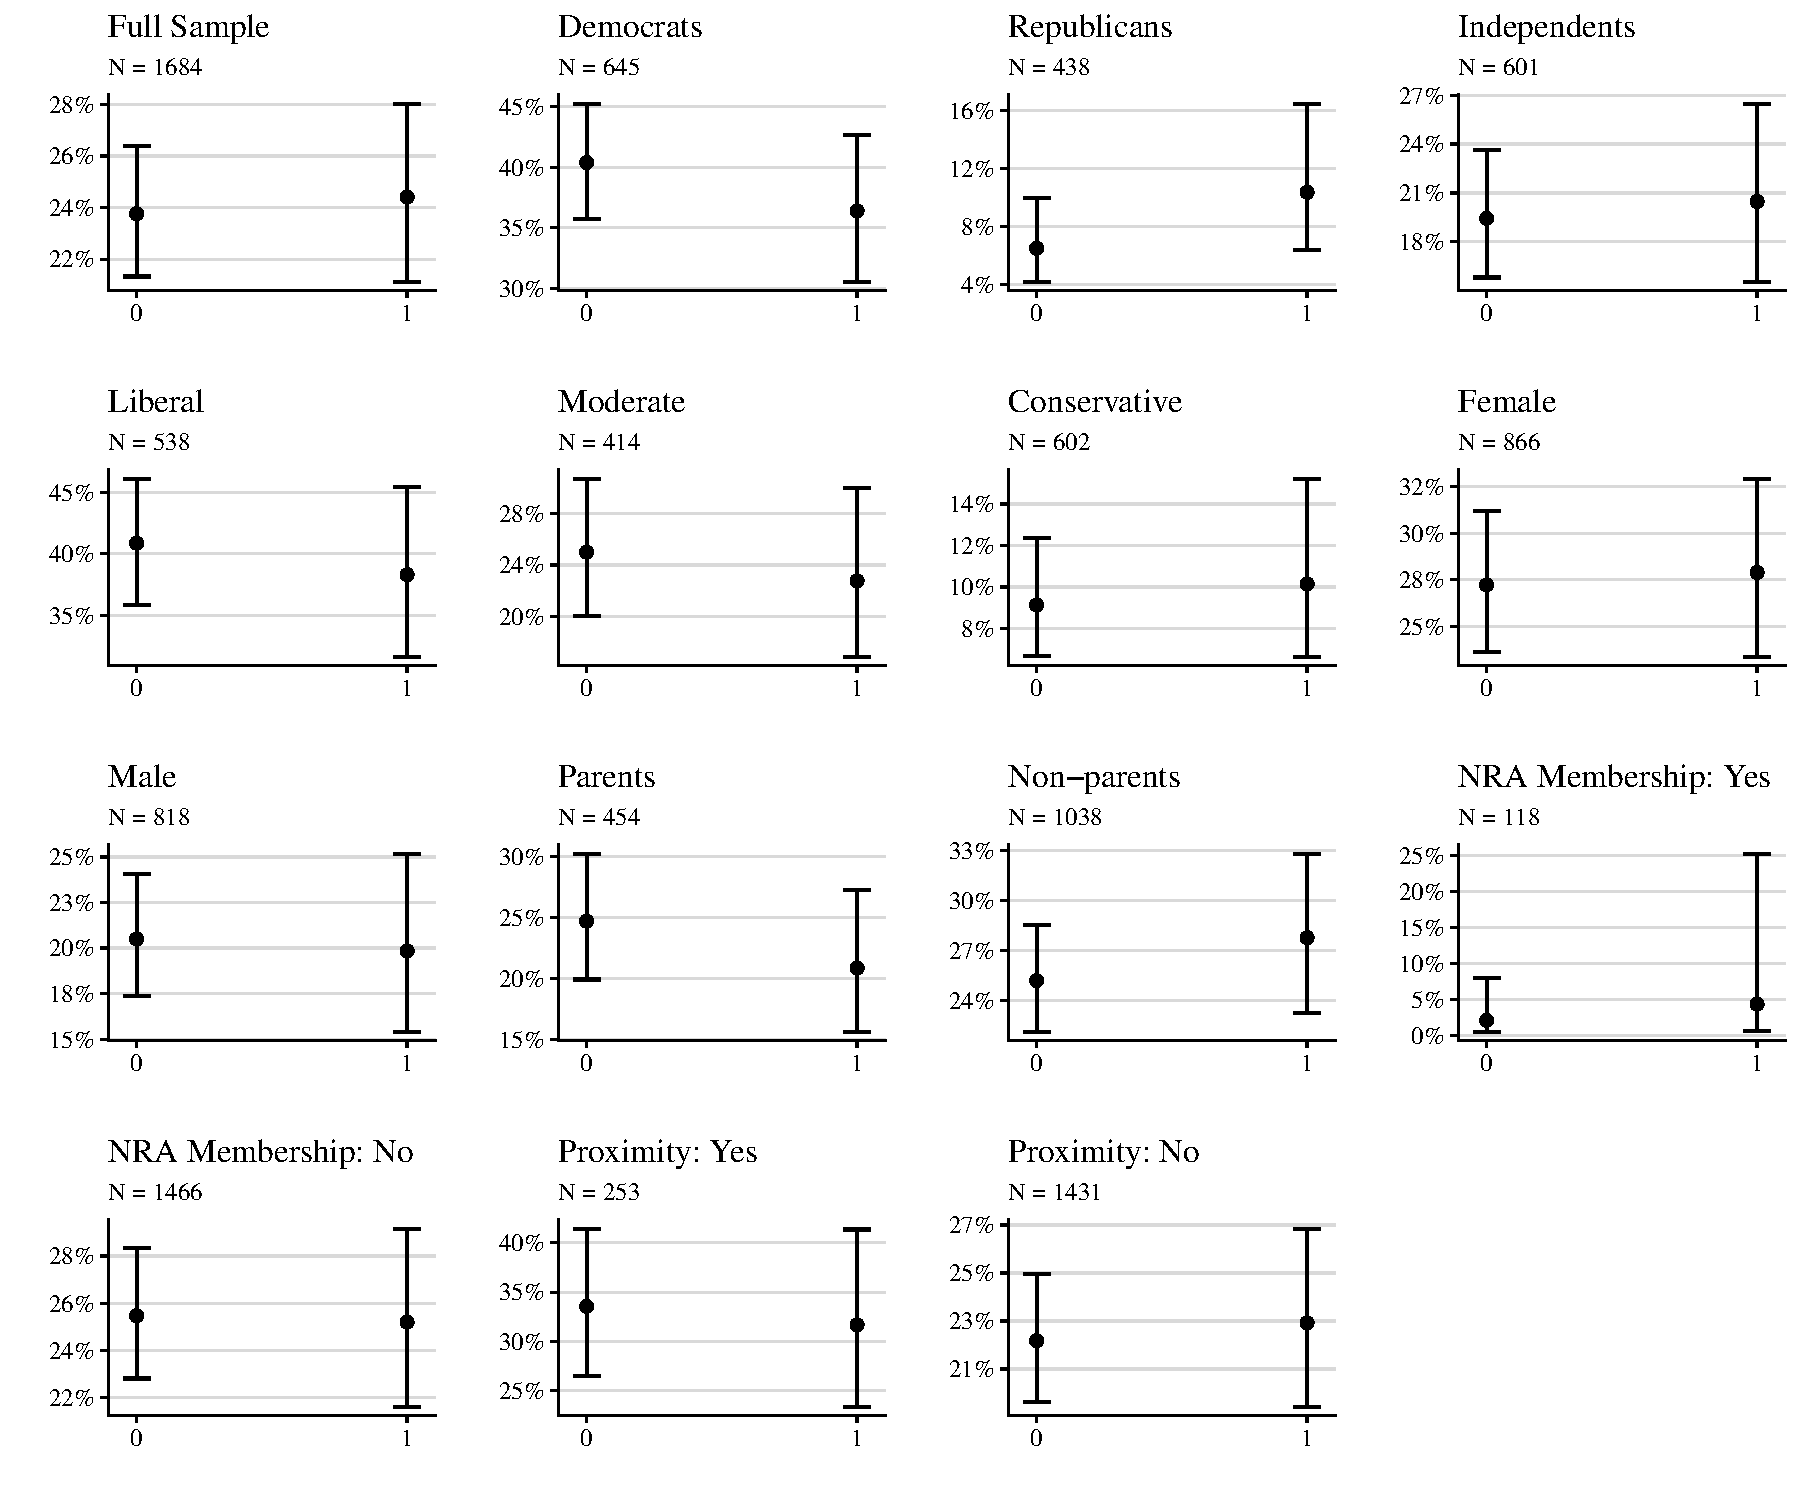
\includegraphics[width = 0.9\linewidth]{/Users/mz/Box/repository/replication/rogowski_tucker_2019_psrm/figs/fig1.pdf}
\captionsetup{justification = raggedright, singlelinecheck = false}
\caption{Predicted probabilities of gun control support (support = 1) before and after the 2012 Sandy Hook shooting. In the \(x\)-axis, 0 means pre-event and 1 means post-event. The error bars show the 95\% confidence interval.}\label{fig1}
\end{figure}
% latex table generated in R 4.0.0 by xtable 1.8-4 package
% Wed May 13 22:27:16 2020
\begin{table}[ht]
\centering
\caption{Effect of the Sandy Hook Shooting on Gun Control Support (5-points Likert Scale), Ordered Logit Results} 
\label{tab1}
\begin{tabular}{lccrrr}
  \toprule
 & Estimate & Standard Error & \(z\)-statistic & \(p\)-value & \(N\) \\ 
  \midrule
Full Sample & 1.144 & 0.091 & 1.475 & 0.140 & 1684 \\ 
  Democrats & 0.892 & 0.145 & $-$0.788 & 0.431 & 645 \\ 
  Republicans & 1.524 & 0.200 & 2.109 & 0.035 & 438 \\ 
  Independents & 1.169 & 0.154 & 1.013 & 0.311 & 601 \\ 
  Liberal & 0.923 & 0.161 & $-$0.496 & 0.620 & 538 \\ 
  Moderate & 1.002 & 0.180 & 0.010 & 0.992 & 414 \\ 
  Conservative & 1.495 & 0.168 & 2.388 & 0.017 & 602 \\ 
  Female & 1.036 & 0.124 & 0.287 & 0.774 & 866 \\ 
  Male & 1.174 & 0.137 & 1.169 & 0.242 & 818 \\ 
  Parents & 1.019 & 0.170 & 0.110 & 0.912 & 454 \\ 
  Non-parents & 1.148 & 0.119 & 1.160 & 0.246 & 1038 \\ 
  NRA Membership: Yes & 0.830 & 0.812 & $-$0.229 & 0.819 & 118 \\ 
  NRA Membership: No & 1.083 & 0.098 & 0.820 & 0.412 & 1466 \\ 
  Proximity: Yes & 1.079 & 0.226 & 0.336 & 0.737 & 253 \\ 
  Proximity: No & 1.129 & 0.100 & 1.208 & 0.227 & 1431 \\ 
   \bottomrule
 \multicolumn{5}{l} {\footnotesize Estimates (but not standard errors) exponentiated. Cut point estimates omitted.}
\end{tabular}
\end{table}


\end{document}